\documentclass{report}
\usepackage{amsmath,caption,float,geometry,titlesec,tikz,tkz-euclide,amssymb}
% \documentclass[12pt]{report}

\usepackage{amsmath,amssymb,amsthm,bm,caption,enumitem,float,geometry,graphicx}
\usepackage{hyperref,mathrsfs,titlesec,tikz,tkz-euclide,wrapfig}

\usepackage[math]{cellspace}
\geometry{a4paper, margin=1in}

\hypersetup{hidelinks}
%\hyphenpenalty=10000

\title{Projective Geometry}
\author{Tejaswi K, Niti Torphe, Ruchith R, Saroj Kumar \and Supervisor: Dr. Steven Spallone}
\date{}

\titleformat{\chapter}
    [frame]
    {\bfseries\Huge}
    {\Large CHAPTER \thechapter}
    {1ex}{\centering}[]

\DeclareCaptionFormat{capfmt}{\textbf{#1 #2}#3}
\captionsetup{format=capfmt}

\newtheorem{theorem}{Theorem}
\newtheorem{prop}{Proposition}
\newtheorem{lemma}{Lemma}

\theoremstyle{definition}
\newtheorem{definition}{Definition}
\newtheorem*{ex}{Ex}

\theoremstyle{remark}
\newtheorem*{notation}{Notation}
\newtheorem*{remark}{Remark}

\newcommand\conop{\oplus_{\vphantom{\dfrac{}{}}O}}
\newcommand\tgrp[3]{\mathrm{#1}_{#2}(\mathbb{#3})}
\newcommand\SO[2]{\tgrp{SO}{#1}{#2}}
\newcommand\AffF[2]{\mathbb{A}^{#1}(\mathbb{#2})}
\newcommand\Aff[1]{\mathbb{A}^{#1}}
\newcommand\norm[1]{\left\lVert{#1}\right\rVert}

\newcommand{\R}{\mathbb{R}}
\newcommand{\Q}{\mathbb{Q}}
\newcommand{\Z}{\mathbb{Z}}
\newcommand{\C}{\mathbb{C}}
\newcommand{\N}{\mathbb{N}}
\newcommand{\F}{\mathbb{F}}
\newcommand{\Ps}{\mathbb{P}}

\renewcommand\qedsymbol{$\blacksquare$}

\DeclareMathOperator{\A}{A}
\DeclareMathOperator{\GA}{GA}
\DeclareMathOperator{\GL}{GL}
\DeclareMathOperator{\Hom}{Hom}
\DeclareMathOperator{\End}{End}
\DeclareMathOperator{\Prj}{P}
\DeclareMathOperator{\ch}{ch}

\setlength{\cellspacetoplimit}{5pt}
\setlength{\cellspacebottomlimit}{5pt}

\addtocontents{toc}{\protect\setcounter{tocdepth}{1}}

%% tejaswi
%%
%%\documentclass[a4paper,12pt]{report}
%%\usepackage{amsmath,amsthm,amssymb,graphicx,float,tikz,tkz-euclide,geometry,hyperref}
%%
%%\hypersetup{hidelinks}
%%
%%\hyphenpenalty=10000
%%
%%\newtheorem*{theorem}{Theorem}
%%\newtheorem*{prop}{Proposition}
%%\newtheorem*{lemma}{Lemma}
%%
%%\theoremstyle{definition}
%%\newtheorem*{definition}{Definition}
%%\newtheorem*{ex}{Ex}
%%
%%\theoremstyle{remark}
%%\newtheorem*{remark}{Remark}
%%
%%\renewcommand\qedsymbol{$\blacksquare$}
%%
%%\newcommand{\R}{\mathbb{R}}
%%\newcommand{\Q}{\mathbb{Q}}
%%\newcommand{\Z}{\mathbb{Z}}
%%\newcommand{\C}{\mathbb{C}}
%%\newcommand{\N}{\mathbb{N}}
%%\newcommand{\F}{\mathbb{F}}
%%
%%\addtocontents{toc}{\protect\setcounter{tocdepth}{1}}

\begin{document}

\title{Projective Geometery}
\author{Ruchith R}
\date{}

\section*{Reference Formuale}
Focus : $(ae,0)$

\noindent
Directrix : $x = \frac{a}{e}$
\subsection*{Parabola $(e = 1)$}

Equation : $$y^2 = 4ax$$

\noindent
Parametric form : $(at^2,2at)$

\subsection*{Ellipse $(0 < e < 1)$}
Equation : $$\frac{x^2}{a^2} + \frac{y^2}{b^2} = 1$$

\noindent
Parametric form : $(a\cos t,b\sin t)$

\subsection*{Hyperbola $(e > 1)$}
Equation : $$\frac{x^2}{a^2} - \frac{y^2}{b^2} = 1$$

\noindent
Parametric form : $(a\sec t,b\tan t)$

\section*{Group law on Parabola}

Given any parabola, there exists an affine transformation that takes it to the curve $y = x^2$.
\begin{figure}[H]
    \centering
    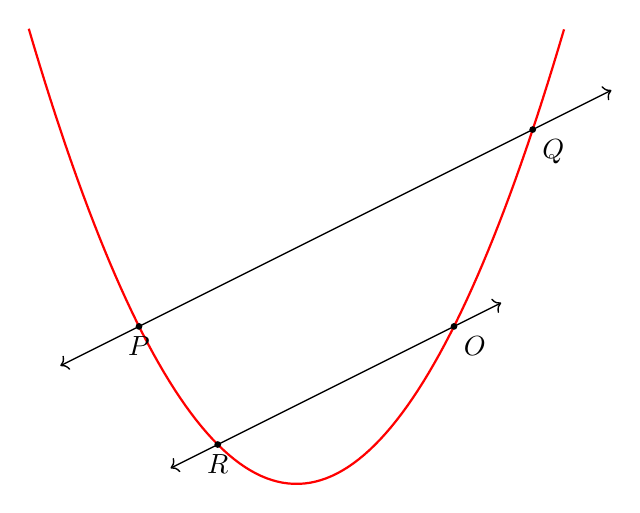
\begin{tikzpicture}[scale=2]
        \draw[thick,red,domain=-1.7:1.7,samples=100] plot (\x,{(\x)^2});
        \tkzDefPoint(1,1){O}
        \tkzDefPoint(-0.5,0.25){R}
        \tkzDefPoint(-1,1){P}
        \tkzDefPoint(1.5,2.25){Q}
        
        \tkzDrawLine[<->,line width=0.5,add=0.2 and 0.2](P,Q)
        \tkzDrawLine[<->,line width=0.5,add=0.2 and 0.2](O,R)
        
        \tkzDrawPoints[fill=black](O,P,Q,R)
        \tkzLabelPoints[below right](O)
        \tkzLabelPoints[below](P)
        \tkzLabelPoints[below right](Q)
        \tkzLabelPoints[below](R)
    \end{tikzpicture}
    \caption{$R = P\oplus Q$}
\end{figure}

We define the parametric coordinates of the point $R$ as $(r,r^2)$.
We compare the slopes of the two lines $PQ$ and $OR$ to obtain the co-ordinates of $R$.
\[\frac{r^2-o^2}{r-o} = \frac{p^2-q^2}{p-q}\]
\[r = p+q-o\]
We define a homomorphism from the points on the parabola to R as $\phi((x,x^2)) = x-o$.
The map that is defined is a bijection hence it is an isomorphism.
The curve shown in the figure is $\mathbb{R}^2$ however the algebra performed remains the same if the field is changed to $\mathbb{C}^2$ .

\section*{Solving for curves in finite fields}

We first investigate the solution set of a curve when working with finite field $\mathbb{Z}_p$.
\[\mathcal{C}  = \{(x_1,x_2,\cdots,x_n) \in \mathbb{Z}_p^n \text{ }|\text{ } condition \} \subseteq \mathbb{Z}_p^n\]
We notice that $\mathbb{Z}_p^n$ contains a finite number of points ($p^n$) and so will $V$.
So it is a valid approach to just verify which points out of these will satisfy the condition.
\vspace{1ex}

\noindent
We now see the solution for one such problem
\[V = \{(x,y,z) \in \mathbb{Z}_p^3 \text{ }| x^2+y^2 = z^2\}\]
We take a different approach to the problem.
We set $z$ as a parameter and plot the various curves for different values of $z$.
Now the problem is simplified to two variables for each value of $z$.
We see that we can embed $\mathbb{Z}_p^2 \text{ in } \mathbb{R}^2$ such that $\mathbb{Z}_p^2 \subset \mathbb{R}^2$.

For every $z \in \mathbb{Z}_p$, 
Define $\mathcal{V}_z = \{(x,y) \text{ }| x^2+y^2=z^2\}$

Notice that: 
\[V = \bigcup_{z \in \mathbb{Z}_p}\mathcal{V}_z\cap\mathbb{Z}_p^2 \]
\begin{figure}[H]
    \centering
    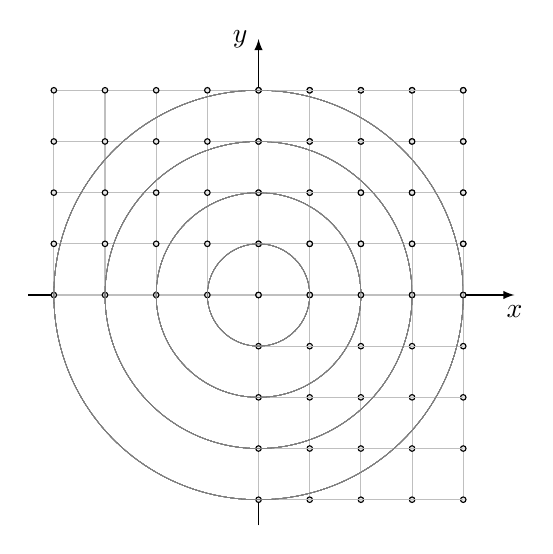
\begin{tikzpicture}[scale=0.65]
        \tkzInit[xmin=-4.5,xmax=4.5,ymin=-4.5,ymax=4.5]
        \tkzDrawX
        \tkzDrawY
        \foreach \x in {0,...,4} {
            \draw[gray!50] (\x,-4) -- (\x,4);
            \draw[gray!50] (-4,\x) -- (4,\x);
            \foreach \y in {-4,...,4} {
                \tkzDefPoint(\x,\y){P\x\y}
                \tkzDrawPoint(P\x\y)
            }
            \tkzDefPoints{0/0/A,1/0/a,2/0/b,3/0/c,4/0/d}
            \tkzDrawCircles(A,a A,b A,c A,d)
          }
          \foreach \x in {-4,...,4} {
            \draw[gray!50] (\x,0) -- (\x,4);
            \draw[gray!50] (0,\x) -- (4,\x);
            \foreach \y in {0,...,4} {
                \tkzDefPoint(\x,\y){P\x\y}
                \tkzDrawPoint(P\x\y)
            }
            \tkzDefPoints{0/0/A,1/0/a,2/0/b,3/0/c,4/0/d}
            \tkzDrawCircles(A,a A,b A,c A,d)
          }
    \end{tikzpicture}
    \caption{The figure represents the $\mathbb{Z}_5$ solutions}
\end{figure}

\section*{Desargues’ Theorem}
There are two triangles $\varDelta ABC$ and $\varDelta XYZ$ in in three dimensional space.
If the lines AX,BY and CZ meet at a point, then the points formed from joining lines AB,BC,AC with PQ,QR,PR respectively are collinear.

\section*{Group Law on Cubics}

  We have a projective cubic curve $\mathcal{C}$ with a given point $O$ on it.
  The addition law is defined as follows:

  To add P and Q, take the third intersection point $P*Q$, join it to $O$ by a line, and then take the third intersection point to be $P+Q$. In other words, set $P + Q$ = $O*(P*Q)$
  In case of $P=Q$, the line passing through $P$ and $Q$ is taken to be the tangent to $\mathcal{C}$ at $P$.

  \begin{figure}[H]
    \centering
    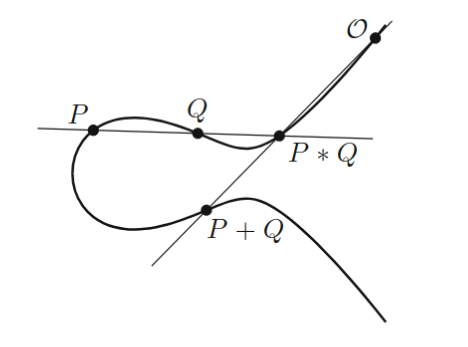
\includegraphics[width=0.5\linewidth]{Grouplaw.png}
  \end{figure}

  In short, we consider a point to intersect a line twice if it is tangent to the curve and thrice if the point is an inflection point. 
  
  Notice that:
  \[P*Q=R\Longleftrightarrow  Q*R=P \Longleftrightarrow R*P=Q\]
  Now we verify that the above addition rule with the set of points on $\mathcal{C}$ does indeed form a group.

  \subsection*{Closure}
  We first see that the set is closed under the operation $*$.
  From Bezout's theorem we can say that given two points on $\mathcal{C}$, there is a third point that intersects with the curve and line through the previous point which proves $\mathcal{C}$ is closed under $*$.
  Thus, for any two points $P$ and $Q$ that lie on $\mathcal{C}$, $P+Q := O*(P*Q)$ also lies on $\mathcal{C}$.

  \subsection*{Identity}
  For any $P$,we have
  \[P+O = O*(O*P) = P\]
  Which shows that $O$ is the identity element and it belongs to $\mathcal{C}$
  
  \subsection*{Inverse}
  Let $S:=O*O$.
  For any point $Q$, consider $Q+(Q*S)$
  \[Q+(Q*S) = O*(Q*(Q*S)) = O*S = O\]
  $(Q*S)$ exists if $S$ exists which it must due to Bezout's theorem.
  If $O$ is an inflection point then $S = O$.
  Thus, the inverse of $Q$ is $(Q*S)$ which lies on $\mathcal{C}$

  \subsection*{Associativity}
  We define the following sets of lines:
  \begin{align*}
    l_1 &: \text{Passes through }Q,R,Q*R \\
    l_2 &: \text{Passes through }O,P*Q,P+Q \\
    l_3 &: \text{Passes through }P,Q+R \\
%   \end{align*}
%   \begin{align*}
    m_1 &: \text{Passes through }P,Q,P*Q \\
    m_2 &: \text{Passes through }O,Q*R,Q+R \\
    m_3 &: \text{Passes through }R,P+R
  \end{align*}
  Because the curve is in the projective plane, the point of intersection of lines $l_3$ and $m_3$ always exists and let that point be $T$.
  Now we consider two cubic curves:
  \[L:l_1 l_2 l_3 \text{ and } M:m_1m_2m_3\]
  The two cubics meet at at 9 points:
  \[O,P,Q,R,P*Q,Q*R,P+Q,Q+R,T\]
  \begin{figure}[H]
    \centering
    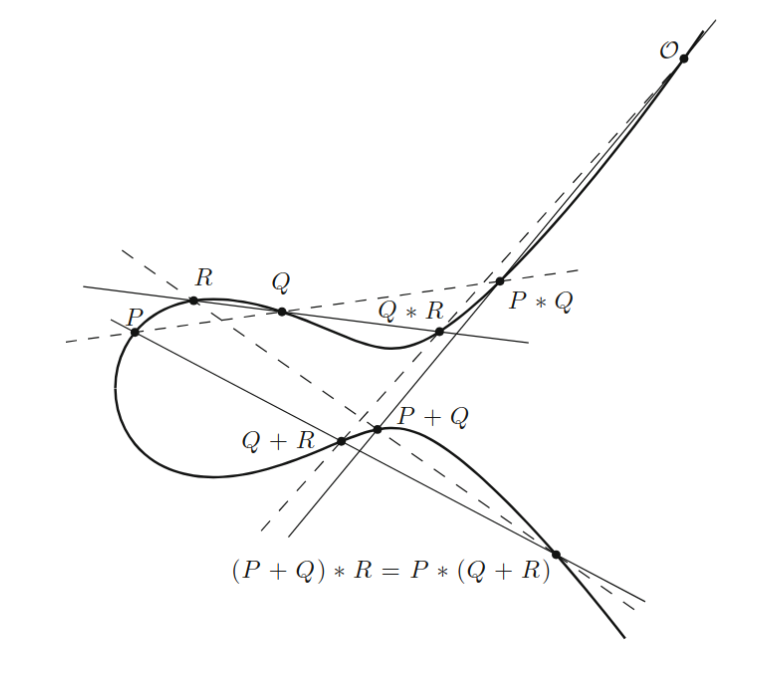
\includegraphics[width=0.7\linewidth]{Associativity.png}
    \caption{Solid lines represents $L$ while dotted lines represents $M$}
  \end{figure}
  But we see that the cubic curve $\mathcal{C}$ passes through all these points except $T$.
  From the Cayley-Bacharach theorem, we have that if two cubic curves $L$ and $M$ intersect at 9 points and another cubic curve $\mathcal{C}$ passes through 8 of those points then it passes through the ninth.
  Hence we can say that $T$ lies on $\mathcal{C}$.
  
  \noindent
  Consider the points of intersection between $\mathcal{C}$ and $l_3$.
  $P$ and $Q+R$ lie on both thus the third point of intersection will be $P*(Q+R)$ which happens to be $T$.

  \noindent
  Similarly, looking at the  points of intersection between $\mathcal{C}$ and $m_3$ we see that point $T$ also happens to be $(P+Q)*R$.

  \noindent
  Because they are the same point, we have that:
  \[(P+Q)*R = P*(Q+R)\]
  From which we can conclude
  \[(P+Q)+R = P+(Q+R)\]
\end{document}